\documentclass{article}
\usepackage{tikz}
\usepackage{quantikz}
\usepackage{braket}
% \usepackage[braket, qm]{qcircuit}
% \usepackage{graphicx}
\usepackage[margin=1in]{geometry}
\usepackage{enumitem}
\usepackage{float}

\graphicspath{{./Images/}}

\title{Introduction to Quantum Information and Quantum Computing\\Assignment 1}
\author{Manuel Santos - 2019231352}
\date{November 2025}

\begin{document}

\maketitle


% ========== 
\section*{Introduction}
\indent This report presents the solution to Assignment 1 of the Introduction to Quantum Information and Quantum Computing course. 

The goal of this assignment is to illustrate a fundamental feature of quantum mechanics: measurement outcomes do not, in general, possess predetermined values prior to measurement—unless one is willing to accept the possibility of faster-than-light communication.

% ========== 1)
\section{Preparation of a shared state}

Alice (A), Bob (B), and Charlie (C) are separated from each other by a considerable distance. A source (S) has prepared three qubits in the so-called $\ket{\mathrm{GHZ}}$ state, according to the circuit below, and sent one qubit to each of them. As always, the qubits all start in the $\ket{0}$ state before passing through the circuit.

\begin{figure}[H]
    \centering
    % --- Left figure in a minipage ---
    \begin{minipage}{0.49\textwidth}
        \centering
        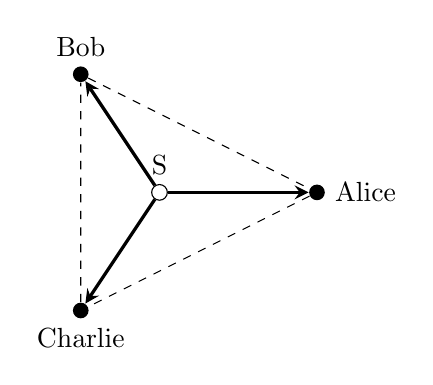
\begin{tikzpicture}[>=stealth, node distance=2cm]
            % Nodes
            \node[fill=black, circle, inner sep=2pt, label=above:{Bob}] (bob) at (0,3) {};
            \node[fill=black, circle, inner sep=2pt, label=right:{Alice}] (alice) at (3,1.5) {};
            \node[fill=black, circle, inner sep=2pt, label=below:{Charlie}] (charlie) at (0,0) {};
            \node[draw, circle, inner sep=2pt, label=above:{S}] (s) at (1,1.5) {};
            % Dashed triangle
            \draw[dashed] (bob) -- (alice) -- (charlie) -- (bob);
            % Solid arrows
            \draw[->, line width=1.2pt] (s) -- (bob);
            \draw[->, line width=1.2pt] (s) -- (charlie);
            \draw[->, line width=1.2pt] (s) -- (alice);
        \end{tikzpicture}
    \end{minipage}
    % \hfill
    % --- Right figure in a minipage ---
    \begin{minipage}{0.49\textwidth}
        \centering
        \begin{quantikz}
            \lstick{$A:$} & \gate{H} & \slice[style=black]{$\ket{\mathrm{Barrier}}$} & & \ctrl{1}  & & \ctrl{2}  & & \slice[style=black]{$\ket{\mathrm{GHZ}}$} & &\\
            \lstick{$B:$} &          &                                      & & \targ{}   & &           & & & &\\
            \lstick{$C:$} &          &                                      & &           & & \targ{}   & & & &
        \end{quantikz}
        % \scalebox{1.0}
        % {
        % \Qcircuit @C=1.0em @R=1.0em { \\
        % \lstick{A :  } & \gate{\mathrm{H}} \barrier[0em]{2}^{\text{\ket{\mathrm{Barrier}}}} & \qw & \ctrl{1} & \ctrl{2} & \qw \barrier[-1em]{2} & \qw\\
        % \lstick{B :  } & \qw & \qw & \targ & \qw & \qw & \qw\\
        % \lstick{C :  } & \qw & \qw & \qw & \targ & \qw & \qw\\}
        % \\}
    \end{minipage}
    \caption{System and circuit representation}
    \label{fig:ex1_system}
\end{figure}

% $\ket{0}$
% $\bra{1}$
% $\braket{0|1}$

\begin{enumerate}[label=(\alph*)]
    % Question A
    \item
    \begin{enumerate}[label=\roman*)]
        \item Let $\ket{\mathrm{Barrier}}$ be the state of the system at the first barrier. Since we start with the qubits $\ket{000}$ ($\ket{\mathrm{CBA}}$ respectively), and we only apply the H gate to the first qubit (A), we get:

        \[
        \ket{000} \xrightarrow{\mathrm{H}_{A}} \ket{00} \left( \frac{\ket{0} + \ket{1}}{\sqrt{2}} \right)
        = \frac{1}{\sqrt{2}} \ket{000} + \frac{1}{\sqrt{2}} \ket{001} = \ket{\mathrm{Barrier}}
        \]

        \item Let $\ket{GHZ}$ be the state of the system at the second barrier (end of the circuit). We start from the $\ket{\mathrm{Barrier}}$ state and apply the CNOT gate first with A as control and B as target, and then with A as control and C as target. As so, we get:

        \[
        \ket{\mathrm{Barrier}} = \frac{1}{\sqrt{2}} \ket{000} + \frac{1}{\sqrt{2}} \ket{001} \xrightarrow{\mathrm{CNOT}_{A,B}} 
        \frac{1}{\sqrt{2}} \ket{000} + \frac{1}{\sqrt{2}} \ket{011} \xrightarrow{\mathrm{CNOT}_{A,C}} 
        \frac{1}{\sqrt{2}} \ket{000} + \frac{1}{\sqrt{2}} \ket{111} = \ket{\mathrm{GHZ}}
        \]
    \end{enumerate}

    At the first barrier, the system is in a superposition of $\ket{000}$ and $\ket{001}$, represented by $\ket{\mathrm{Barrier}}$. After applying the CNOT gates, this superposition is extended across all three qubits, resulting in the maximally entangled state $\ket{\mathrm{GHZ}}$.

    % Question B
    \item Measuring Alice’s qubit collapses its state: 
    \begin{itemize}
        \item If Alice obtains $0$, Bob and Charlie’s qubits collapse to $\ket{00}$
        \item If Alice obtains $1$, Bob and Charlie’s qubits collapse to $\ket{11}$
    \end{itemize}
    
    However, from Bob or Charlie’s perspective alone, their measurement outcomes are still random until they compare results with Alice.

    % Question C
    \item As shown previously, the $\ket{\mathrm{GHZ}}$ state is in a superposition of $\ket{000}$ and $\ket{111}$. Thus, we expect to observe $\ket{000}$ half of the time and $\ket{111}$ the other half.
    
    By running the simulation, we confirm that this is the case, as shown by the results in Figure~\ref{fig:ex1_c}.
    
    \begin{figure}[H]
        \centering
        \includegraphics[width=0.5\textwidth]{Images/1_c.png}
        \caption{Result of the simulation for 1024 shots}
        \label{fig:ex1_c}
    \end{figure}

\end{enumerate}

% ========== 2)
\section{Independent Operations}

After receiving their qubit, Alice, Bob, and Charlie each apply one of two operations to their qubit: either $M_X = H \quad \text{or} \quad M_Y = H S^\dagger$. Immediately afterward, each of them measures their qubit.

\begin{enumerate}[label=(\alph*)]
    \item Let's start with the case in which all of them apply $M_X = H$, to which we'll call state $\ket{\mathrm{XXX}}$. The following circuit generates state $\ket{\mathrm{XXX}}$: 
    % \begin{figure}[H]
    %     \centering
    %     \begin{quantikz}[wire types={q,q,q,c}]
    %         \lstick{$A:$} & \gate{H} & \ctrl{1} & \ctrl{2} & \slice[style=black]{$\ket{\mathrm{GHZ}}$} & & \gate{H} & \slice[style=black]{} & & \meter{} & & &\\
    %         \lstick{$B:$} & & \targ{} & & & & \gate{H} & & & & \meter{} & &\\
    %         \lstick{$C:$} & & & \targ{} & & & \gate{H} & & & & & \meter{} &\\
    %         \lstick{$meas:$} & \qwbundle{3} & & & & & & & & \wire[u][3]{\substack{c \\[2pt] 3}} & \wire[u][2]{c} & \wire[u][1]{c} &
    %     \end{quantikz}        
    %     \caption{Circuit XXX for all applying $M_X = H$}
    %     \label{fig:mx_circuit}
    % \end{figure}

    We expect the $\ket{\mathrm{XXX}}$ state to be:
    
    \begin{equation*}
        \begin{aligned}
            \ket{\mathrm{GHZ}} 
            &= \frac{1}{\sqrt{2}} \ket{000} + \frac{1}{\sqrt{2}} \ket{111} \\
            &\xrightarrow{\mathrm{H}_{A}} \frac{1}{2} \ket{000} + \frac{1}{2} \ket{001} + \frac{1}{2} \ket{110} - \frac{1}{2} \ket{111} \\
            &\xrightarrow{\mathrm{H}_{B}} \frac{1}{2\sqrt{2}} \ket{000} + \frac{1}{2\sqrt{2}} \ket{010} + \frac{1}{2\sqrt{2}} \ket{001} + \frac{1}{2\sqrt{2}} \ket{011} \\
            &\quad \quad + \frac{1}{2\sqrt{2}} \ket{100} - \frac{1}{2\sqrt{2}} \ket{110} - \frac{1}{2\sqrt{2}} \ket{101} + \frac{1}{2\sqrt{2}} \ket{111} \\
            &\xrightarrow{\mathrm{H}_{C}}\frac{1}{2} \ket{000} + \frac{1}{2} \ket{011} + \frac{1}{2} \ket{101} + \frac{1}{2} \ket{110} = \ket{\mathrm{XXX}}
        \end{aligned}
    \end{equation*}

    By running the simulation, we confirm that this is the case, as shown by the results in Figure~\ref{fig:ex2_XXX}.
    
    \begin{figure}[H]
        \centering
        \includegraphics[width=0.5\textwidth]{Images/2_a.png}
        \caption{Result of the simulation of 1024 shots for circuit XXX}
        \label{fig:ex2_XXX}
    \end{figure}

    % Question B
    \item The possible results are $\ket{000}, \ket{011}, \ket{101} \mathrm{and} \ket{110}$ for (C,B,A) = (0,0,0), (0,1,1), (1,0,1), (1,1,0) respectively.
    It's also possible to confirm that in each case, the sum $a+b+c$ is always even.

    % Question C
    \item Next, we considered the circuits in which only one of the participants applies $M_X$ and the others apply $M_Y = HS^\dagger$. 
    
    After simulating these circuits, we observe that only four measurement outcomes are possible for each case, and they are always correlated such that the sum $a+b+c$ is odd.


    % Question D
    \item The possible measurement outcomes for each of these circuits are:

    \begin{itemize}
        \item YYX (Charlie and Bob apply $M_Y$, Alice applies $M_X$): 
        \[
        (C,B,A) = (0,0,1), (0,1,0), (1,0,0), (1,1,1)
        \]
        \begin{figure}[H]
            \centering
            \includegraphics[width=0.5\textwidth]{Images/2_c_YYX.png}
            \caption{Result of the simulation of 1024 shots for circuit YYX}
            \label{fig:ex2_YYX}
        \end{figure}

        \item YXY (Charlie and Alice apply $M_Y$, Bob applies $M_X$): 
        \[
        (C,B,A) = (0,0,1), (0,1,0), (1,0,0), (1,1,1)
        \]
        \begin{figure}[H]
            \centering
            \includegraphics[width=0.5\textwidth]{Images/2_c_YXY.png}
            \caption{Result of the simulation of 1024 shots for circuit YXY}
            \label{fig:ex2_YXY}
        \end{figure}
        
        \item XYY (Alice applies $M_X$, Bob and Charlie apply $M_Y$): 
        \[
        (C,B,A) = (0,0,1), (0,1,0), (1,0,0), (1,1,1)
        \]
        \begin{figure}[H]
            \centering
            \includegraphics[width=0.5\textwidth]{Images/2_c_XYY.png}
            \caption{Result of the simulation of 1024 shots for circuit XYY}
            \label{fig:ex2_XYY}
        \end{figure}
    \end{itemize}
    
    In each case, the sum $a+b+c$ is always odd, as expected from the GHZ correlations.
    
\end{enumerate}


% ========== 
% \section*{Conclusion}



%\sloppy
%\nocite{*}
%\printbibliography


\end{document}
